\documentclass[border=10pt]{standalone}
\usepackage{tikz}\usepackage{amsmath}\usetikzlibrary{arrows.meta}
\begin{document}
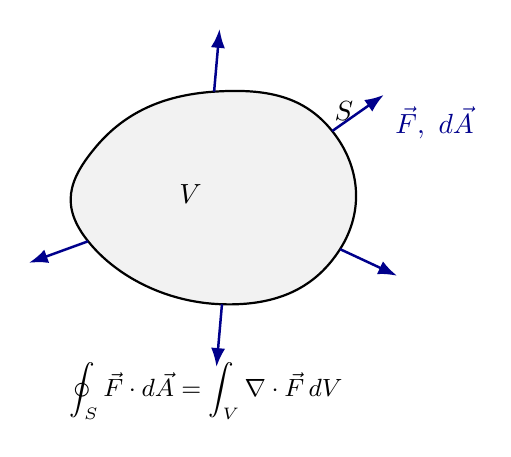
\begin{tikzpicture}[line width=0.9pt,>={Latex[length=2.4mm]}]
  \draw[thick,fill=black!5] plot[smooth cycle,tension=0.8] coordinates {(-1.4,0.7)(0.1,1.4)(1.6,0.9)(1.7,-0.6)(0.2,-1.3)(-1.5,-0.5)};
  \node at (-0.2,0.1){$V$};
  \node at (1.75,1.15){$S$};
  \draw[->,blue!55!black] (1.6,0.9)--++(35:0.8);
  \draw[->,blue!55!black] (1.7,-0.6)--++(-25:0.8);
  \draw[->,blue!55!black] (-1.5,-0.5)--++(200:0.8);
  \draw[->,blue!55!black] (0.1,1.4)--++(85:0.8);
  \draw[->,blue!55!black] (0.2,-1.3)--++(265:0.8);
  \node[blue!55!black] at (2.9,1.0){$\vec F,\ d\vec A$};
  \node at (0,-2.4){\small $\displaystyle\oint_S \vec F\cdot d\vec A=\int_V \nabla\cdot\vec F\,dV$};
\end{tikzpicture}
\end{document}
